\chapter{A Software Solution for the Patrolling Problem}
\label{softwareApplication}

This chapter proposes a web application called \emph{Dronem Web}, based on the \emph{DronemRL} algorithm. The purpose of this platform is to facilitate a way to create, train and share results on multi-robot patrolling problems in the research community. 

\par This application represents an element of originality, as to the best of our knowledge there is no system currently available for manipulating and analyzing MRP environments. One of the strongest points of the proposed software solution is the possibility to fetch already trained cloud \emph{reinforcement learning} Q-tables for different environments, in order to further use them in real applications. 

\par Several popular and highly optimized frameworks were used for building this application on both \emph{backend} and \emph{frontend}, such as OpenAI for creating and managing the MRP environments, Django and Django Rest Framework for managing user and environment data, and ReactJS for creating the application layout and handling user interactions with the application. All this frameworks and libraries will be further detailed in this chapter. 

\par The remainder of chapter is structured as follows. In Section \ref{softDev} we make an analysis of the proposed application from a software development point of view. Section \ref{softOpenAI} shows how the MRP environments are created using the \emph{OpenAI Gym} \cite{brockman2016openai} framework, while in Sections \ref{BE} and \ref{FE} the main \emph{backend} and \emph{frontend} technologies are discussed. Implementation details and design choices are highlighted in Section \ref{implementation} and a user manual is proposed in Section \ref{userManual}. Towards the end of the chapter, some conclusions are drawn in the form of a brief discussion in Section \ref{softDiscussionn}, and finally, possible future enhancements are presented in Section \ref{futureEnh}.
 
\newpage
\section{Software development}\label{softDev}
Software development \cite{ibmSoftDev} implies all the necessary activities regarding  creation, testing and deployment of applications or other types of software. When developing an application a series of activities need to be taken into consideration in order to minimize the possibility of developing applications containing bugs, this series of activities is called a \emph{software development process} \cite{thePragmaticProgrammer}. 
\par The most important activities in Software development are the following:
\begin{itemize}
    \item Identify the need for creating the application.
    \item Planning - discovering the requirements of the application and its functionalities.
    \item Designing - creating a high-level design of the application (main modules, packages, entities, what kind of data will be managed by the application)
    \item Implementation - writing the code of the application.
    \item Testing - ensuring that the application behaves as expected according to the requirements.
    \item Documenting - writing specification for modules and packages easing maintainability of the code and extending the application.
    \item Deployment and maintenance - releasing the application and correcting any error which may appear in the future.
\end{itemize}

\par The need for Software development comes as a natural consequence of the fact that the code is written by humans, making it unreliable, hence a methodology needs to be followed in order to ensure that major bugs do not appear, and minor bugs are identified quickly and fixed. One good example of a disaster which occurred due to a major bug is The Patriot Missile Failure \cite{badBugs}, where on $25^{th}$ of February 1991, 28 American soldiers died because of a floating point arithmetic error.

\subsection{Analysis and design}\label{ad}
This subsection is focusing solely on the methodology defined in Section \ref{softDev}
\subsubsection{The necessity of this application}
While reading papers about different types of MRP problems, it was noticed that there is no application where, as a user, you can  create your own environments and try to apply different operations on them, therefore, an application capable of managing, analyzing MRP environments and sharing results is needed. Also due to the fact that MRP problems have high applicability in real life scenarios such as smart surveillance systems, this application can also serve as a tool to design such useful systems and test their capabilities.

\subsubsection{Planning}
In the planning phase, also known as \emph{collection of requirements}, we have gathered the main functional requirements of the application with the help of a use case diagram which can be observed in Figure \ref{fig:usecase}


\begin{figure*}[!htb]
\centering
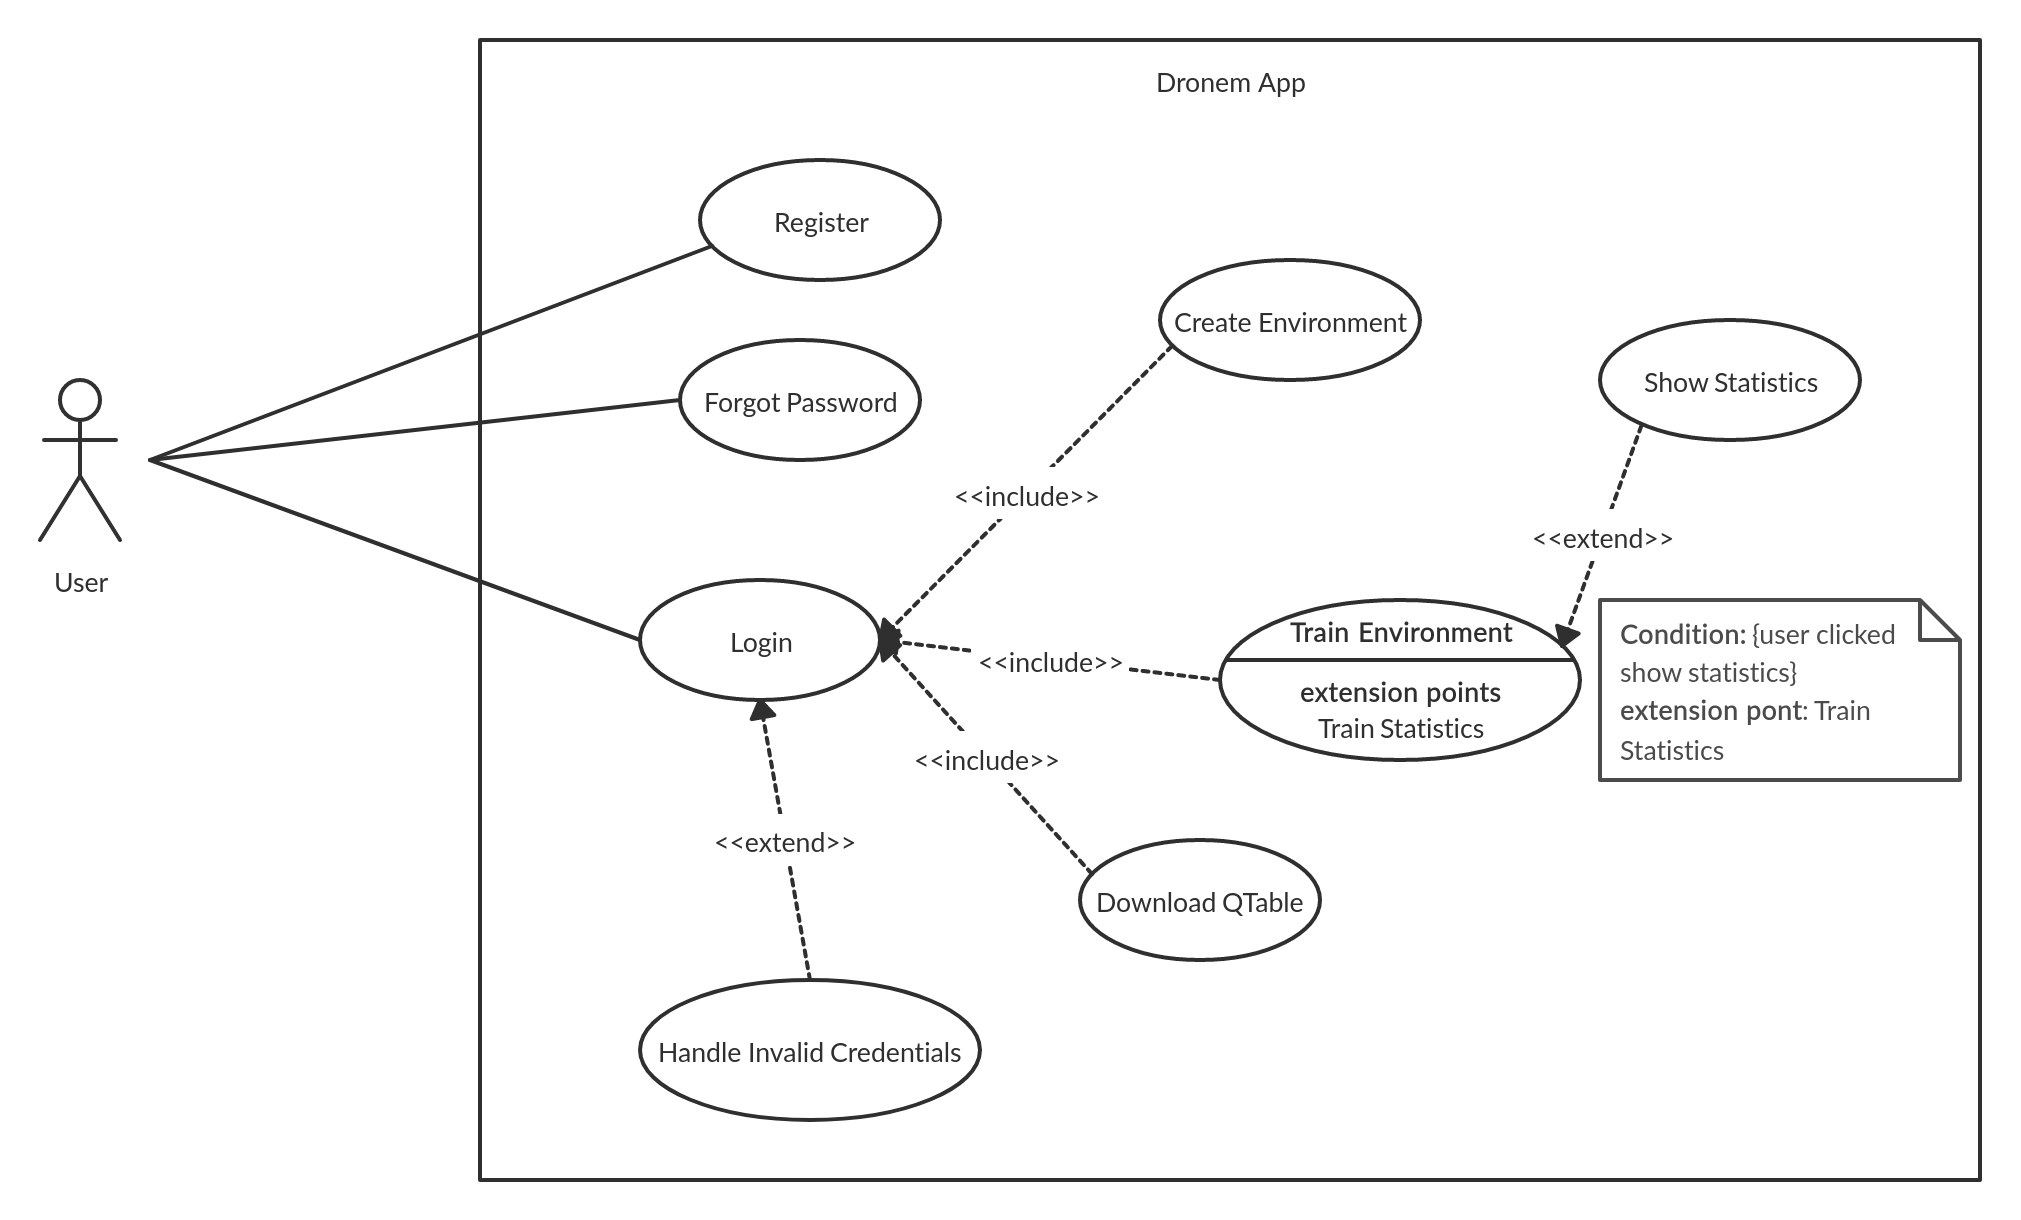
\includegraphics[scale=0.2]{Figures/UseCaseDronemRLFinal.jpg}
\caption{Use case diagram for Dronem web application}
\label{fig:usecase}
\end{figure*}


From the diagram above we can already identify the user as being the only actor of our application and the following use cases:
\begin{itemize}
    \item Register - complete registration flow for becoming a user in the Dronem Web application.
    \item Login - Authentication functionality which provides access to the core features of the application.
    \item Handle Invalid Credentials - verification of user input at login.
    \item Create Environment - use case for creating and managing MRP environments.
    \item Download QTable - possibility to download trained Q-ables for different environments.
    \item Forgot password - resetting password when a user requests it.
    \item Train Environment - possibility to train a MRP environment.
    \item Show Statistics - displaying training statistics for any environment.
\end{itemize}

One other important aspect to note is that, any use case which implies manipulating data, includes \emph{Login} and also, the \emph{Show Statistics} use case makes no sense if an environment was not trained at least once (because until the first training of the environment, there are no statistics)

\subsubsection{Design}
After the \emph{planning} phase where functional requirements were collected, a preliminary model of the main entities and the relationship between them was derived, following the Unified Model Language(UML)\cite{uml} standard, resulting in a conceptual model which can be seen in Figure \ref{fig:conceptualModel}

\begin{figure}[!htb]
    \centering
    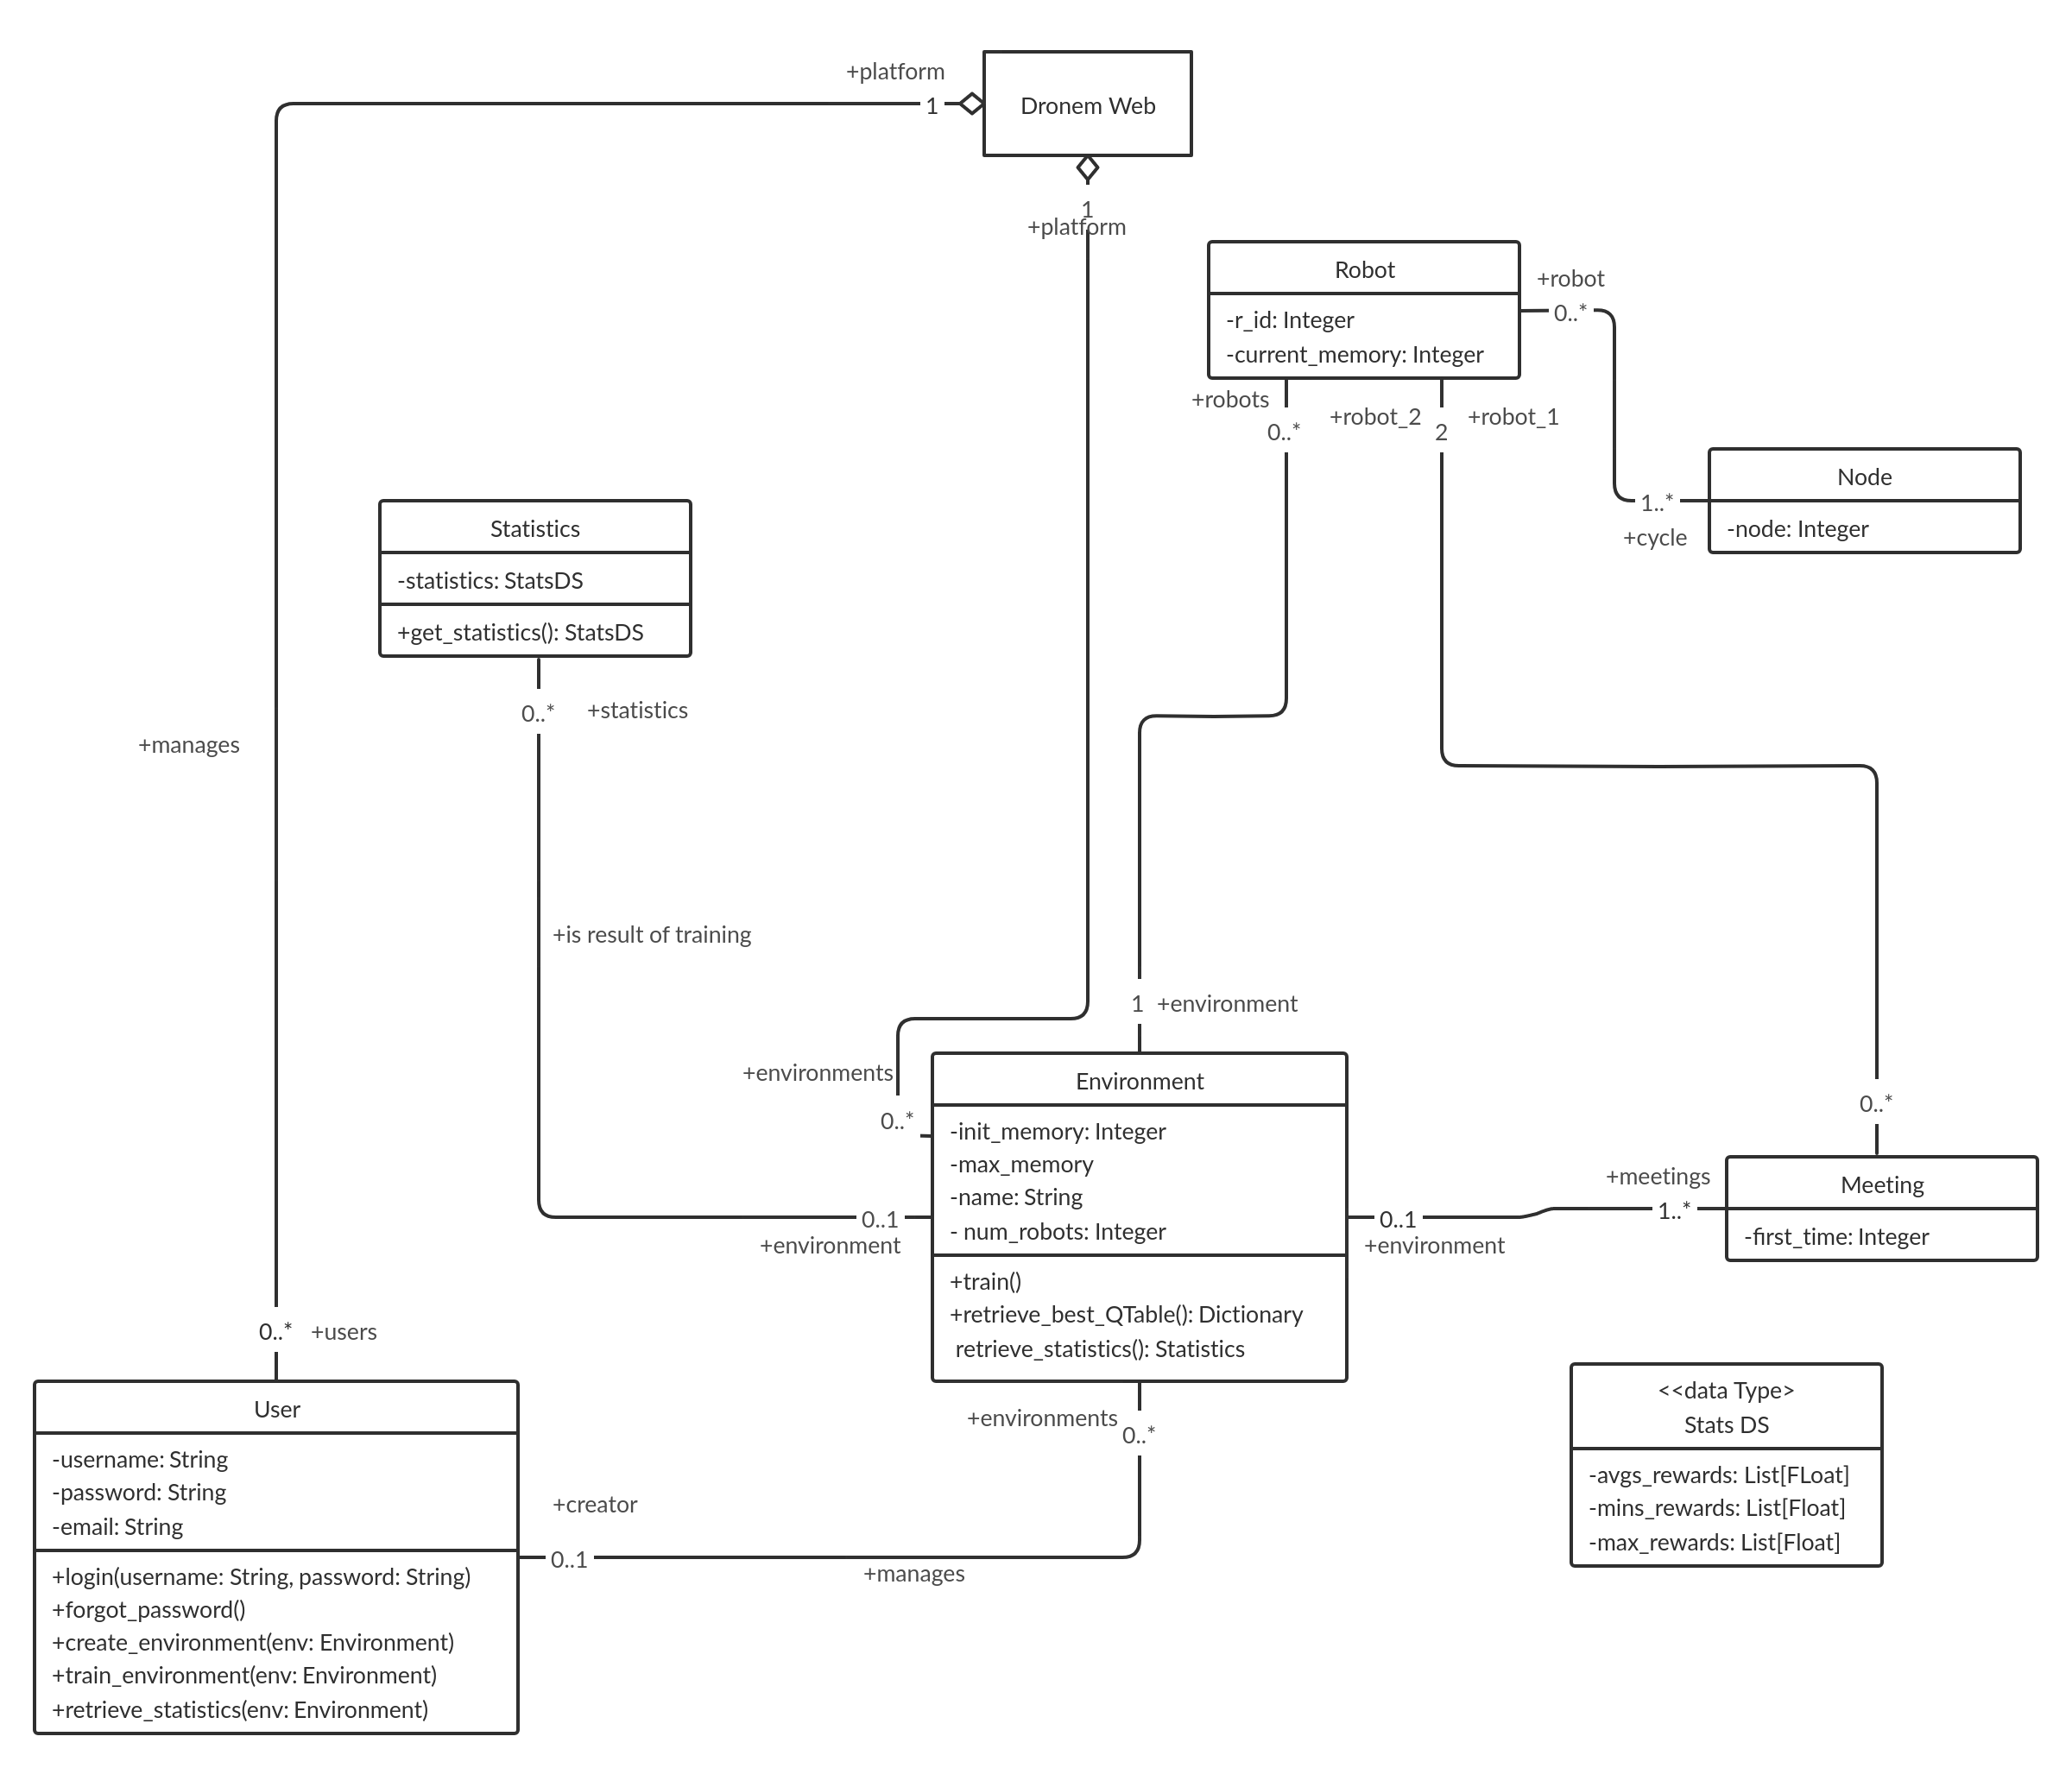
\includegraphics[scale=0.19]{Figures/conceptualModel.jpg}
    \caption{Dronem Web conceptual model}
    \label{fig:conceptualModel}
\end{figure}{}

It is known that one of the biggest problems of software development is the defective communication between clients and developers \cite{communicationProblems}, as usually the actual people who write code are not directly interacting with the client. The conceptual model diagram is an important tool which tries to solve this problems, since it eases the communication between the developers and the client by highlighting the main entities of the application and the interactions between them.
Of course, because diagram presented in Figure \ref{fig:conceptualModel} is just an intermediate step in designing the application, it is not detailed enough in order to start writing code, thus a refinement process was needed in order to obtain the final class diagram which can be viewed in Figure \ref{fig:refineDiag}

\begin{figure}[!htb]
    \centering
    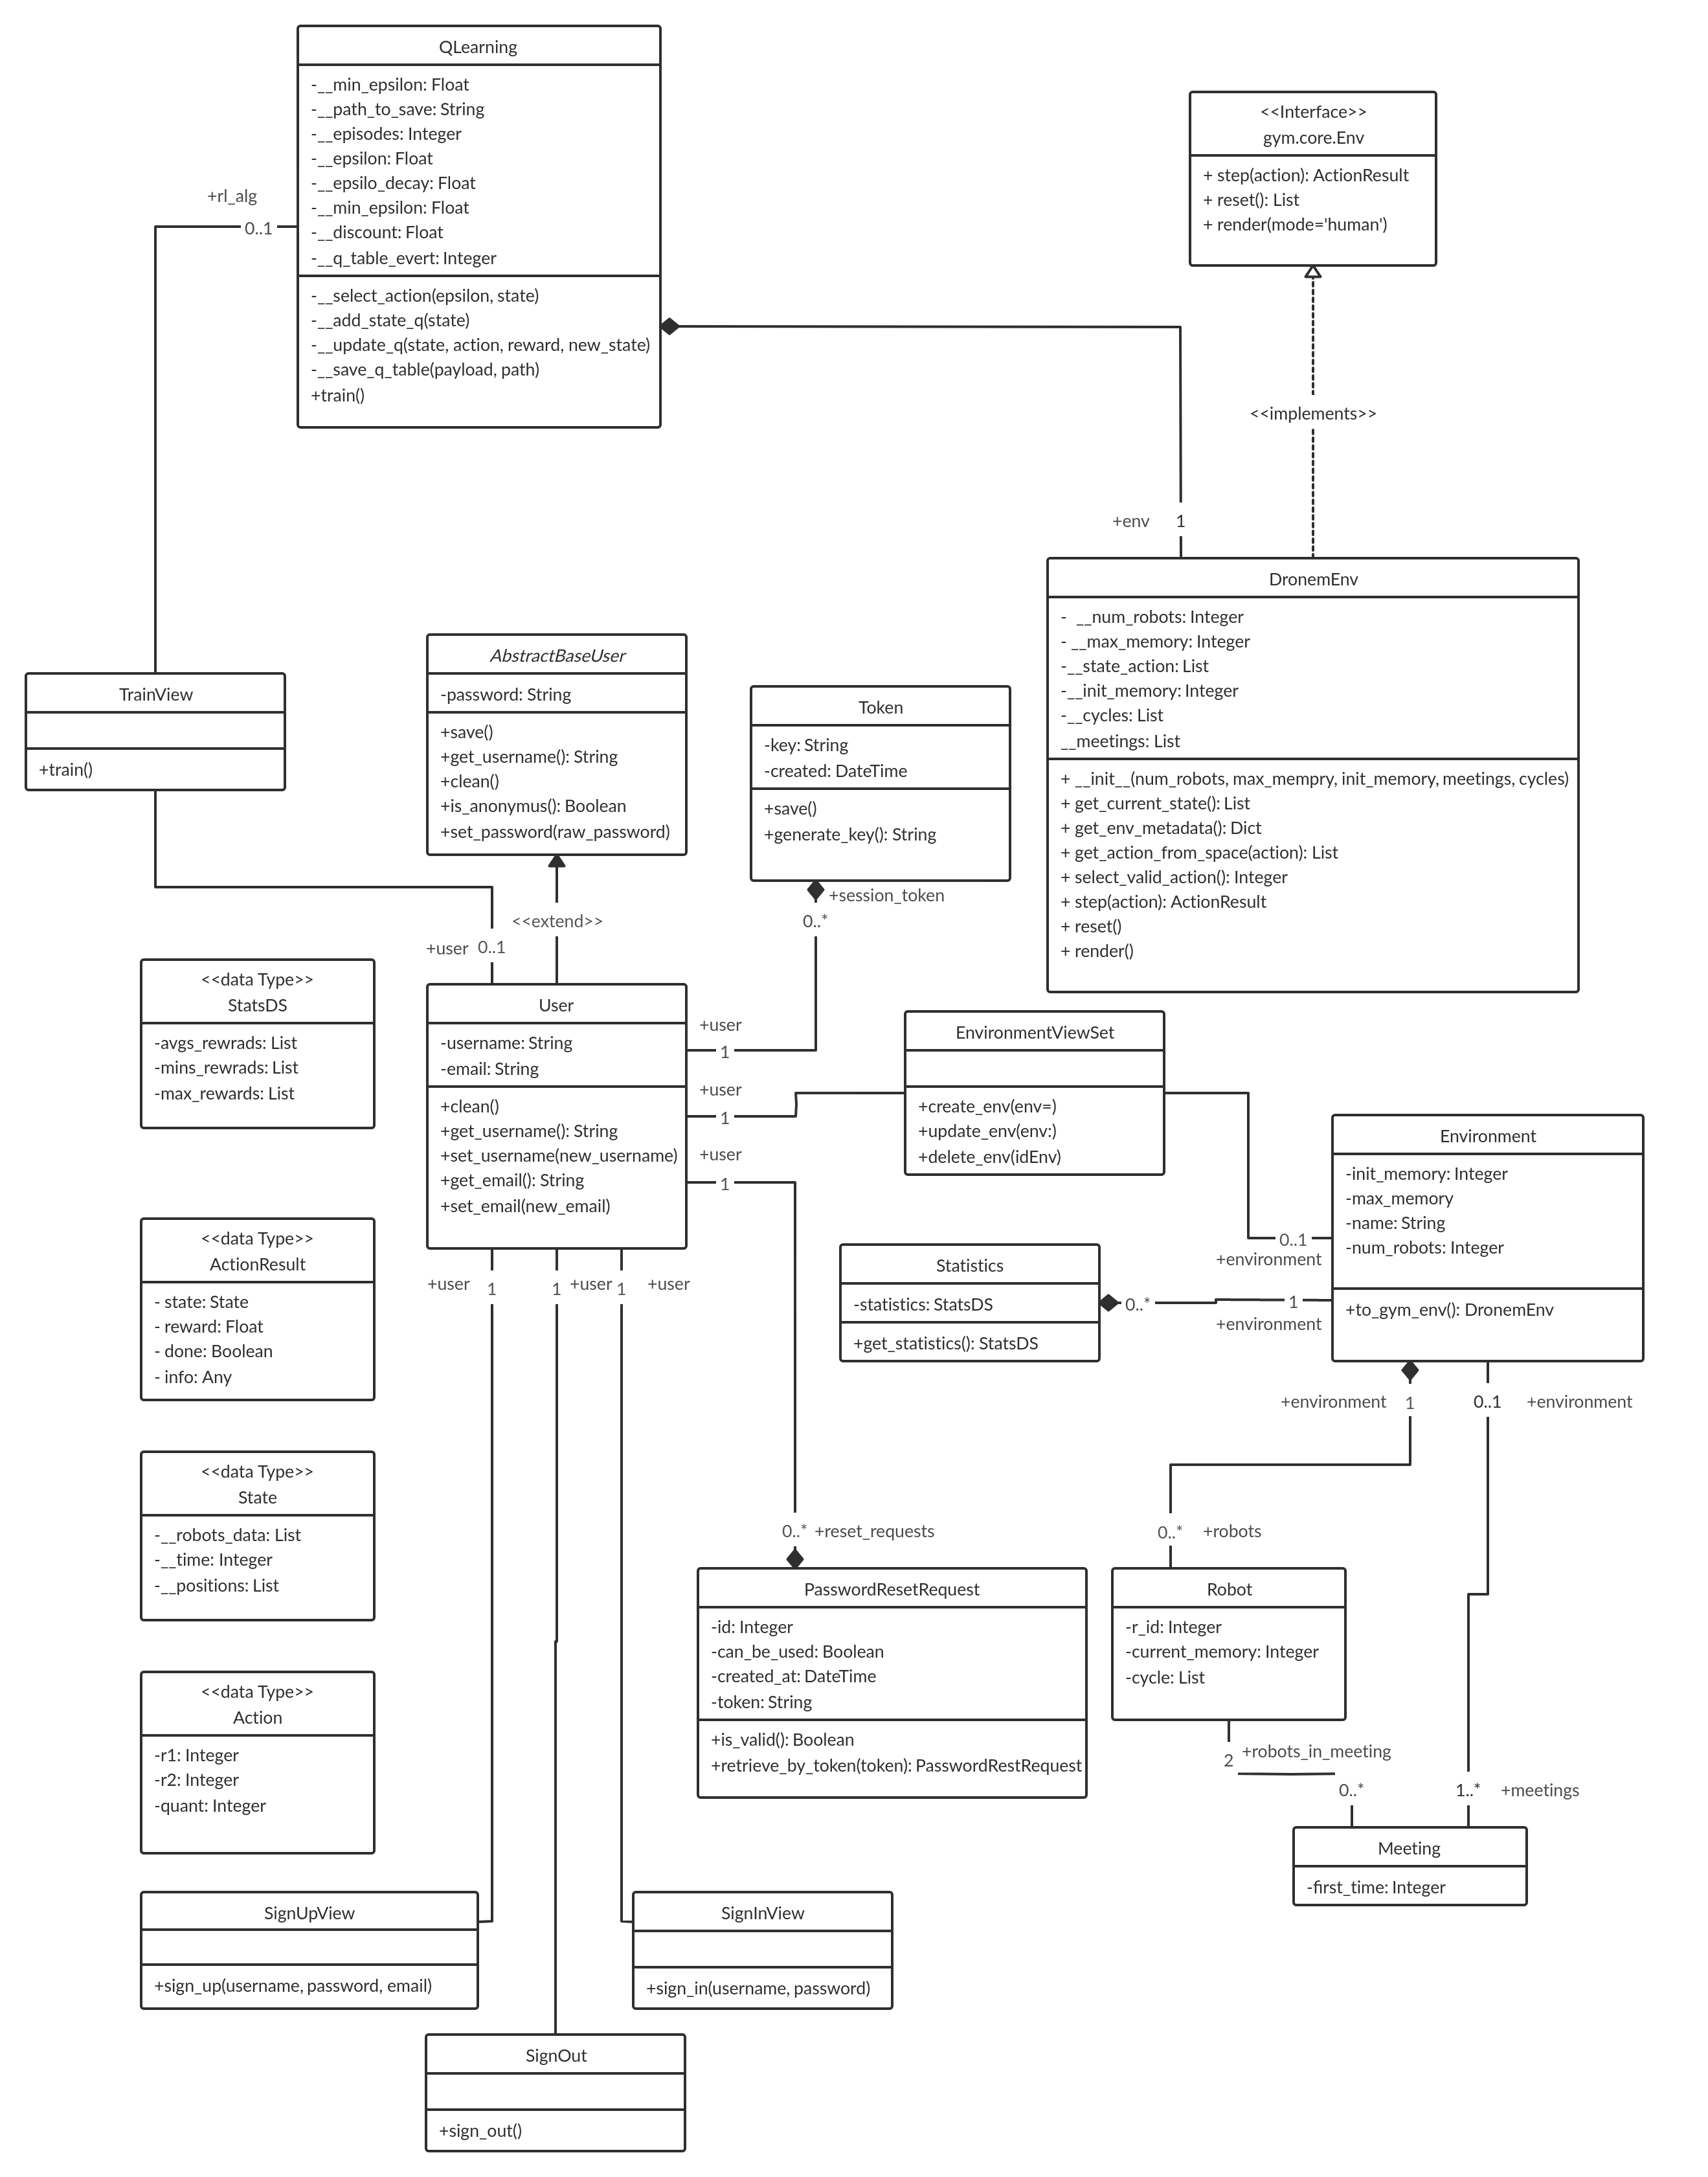
\includegraphics[scale=0.18]{Figures/umlComplete.jpg}
    \caption{Dronem Web refined UML diagram}
    \label{fig:refineDiag}
\end{figure}

\newpage
Having the refined UML class diagram we started implementing the main features of the application. More implementation details together with the next steps in the software development methodology will be outlined in the next sections.

\section{OpenAI}\label{softOpenAI}

 \emph{OpenAI Gym} \cite{brockman2016openai} is a \emph{python} toolkit for reinforcement learning environments which exposes a common interface and an website where researchers can share and compare their results. Reinforcement learning assumes that there is an agent which is situated in an environment. Each step, the agent takes an action, and it receives an observation and reward from the environment. A RL algorithm seeks to maximize some measure of the agent’s total reward, as the agent interacts with the environment. In the RL literature, the environment is formalized as a partially observable Markov decision process \cite{rsab}. OpenAI Gym focuses on the episodic setting of reinforcement learning, where the agent’s experience is broken down into a series of episodes. In each episode, the initial state of the agent is randomly sampled from a distribution, and the interaction proceeds until the environment reaches a terminal state. The goal in episodic reinforcement learning is to maximize the expectation of total reward per episode, and to achieve a high level of performance in as few episodes as possible.


\subsection{The Dronem environment}\label{gymInterface}

The OpenaAI Gym environment for our reinforcement learning model \emph{(Dronem environment)} is constructed upon  the Gym architecture\cite{brockman2016openai}, which is based on the following interface:
\begin{itemize}
  \item \textit{env.reset()} which resets the environment to its initial state;
  \item \textit{env.step(action)} which applies an action to the environment and returns back the new \emph{state} of the environment as an \emph{observation}, a variable called \emph{done} which tells if the episode should end and the \emph{reward} for applying the given action;
  \item \textit{env.render()} which renders the environment;
\end{itemize}


\par As we can see in Figure \ref{fig:dronemEnvPipeline} the life cycle of a Gym Environment is highlighted, by first starting the environment when calling $env.reset()$, then the environment expects an action in order to call $env.step()$, after that we analyze the new state and reward to draw conclusions about our actions. After calling the $env.step()$ function, if the $done$ variable is true, we then stop the Dronem environment.

\par Following the interface defined in Section \ref{gymInterface}, it was easy to design and implement the architecture from Figure \ref{fig:dronemEnvGym} in order to obtain a reinforcement learning environment following the specification of the problem defined in Chapter \ref{flow}. We can observe that we are not limited in the number or type of our parameters and functions used in the environment, as long as we implement the functions in the \emph{Gym} interface.

\begin{figure}[!htb]
    \centering
    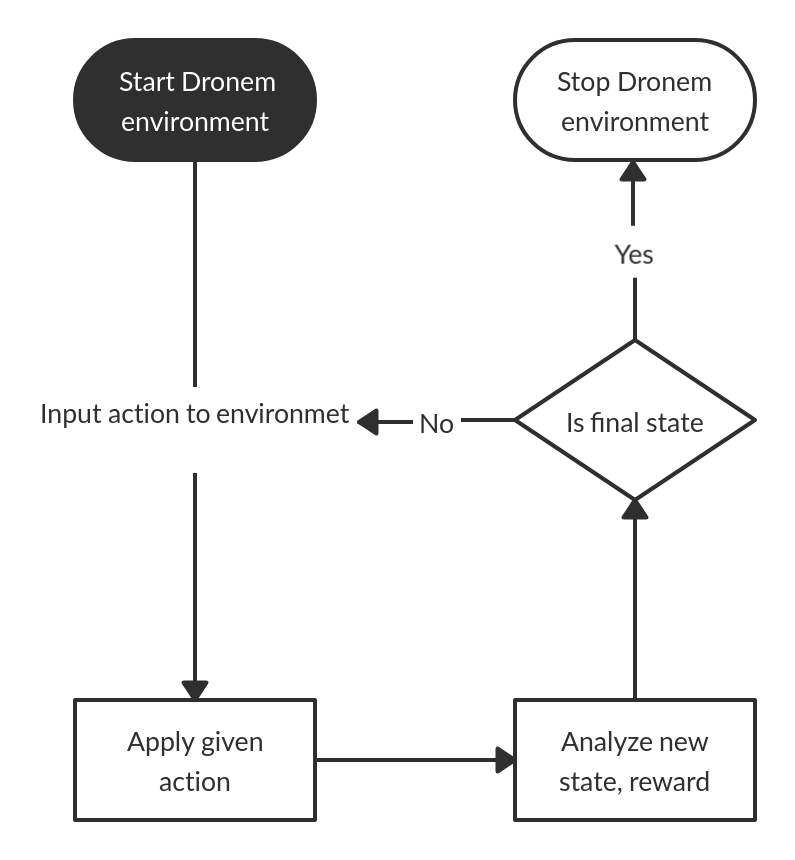
\includegraphics[scale=0.3]{Figures/Gym_env_flow.jpg}
    \caption{Dronem environment life cycle}
    \label{fig:dronemEnvPipeline}
\end{figure}{}

\begin{figure}[!htb]
    \centering
    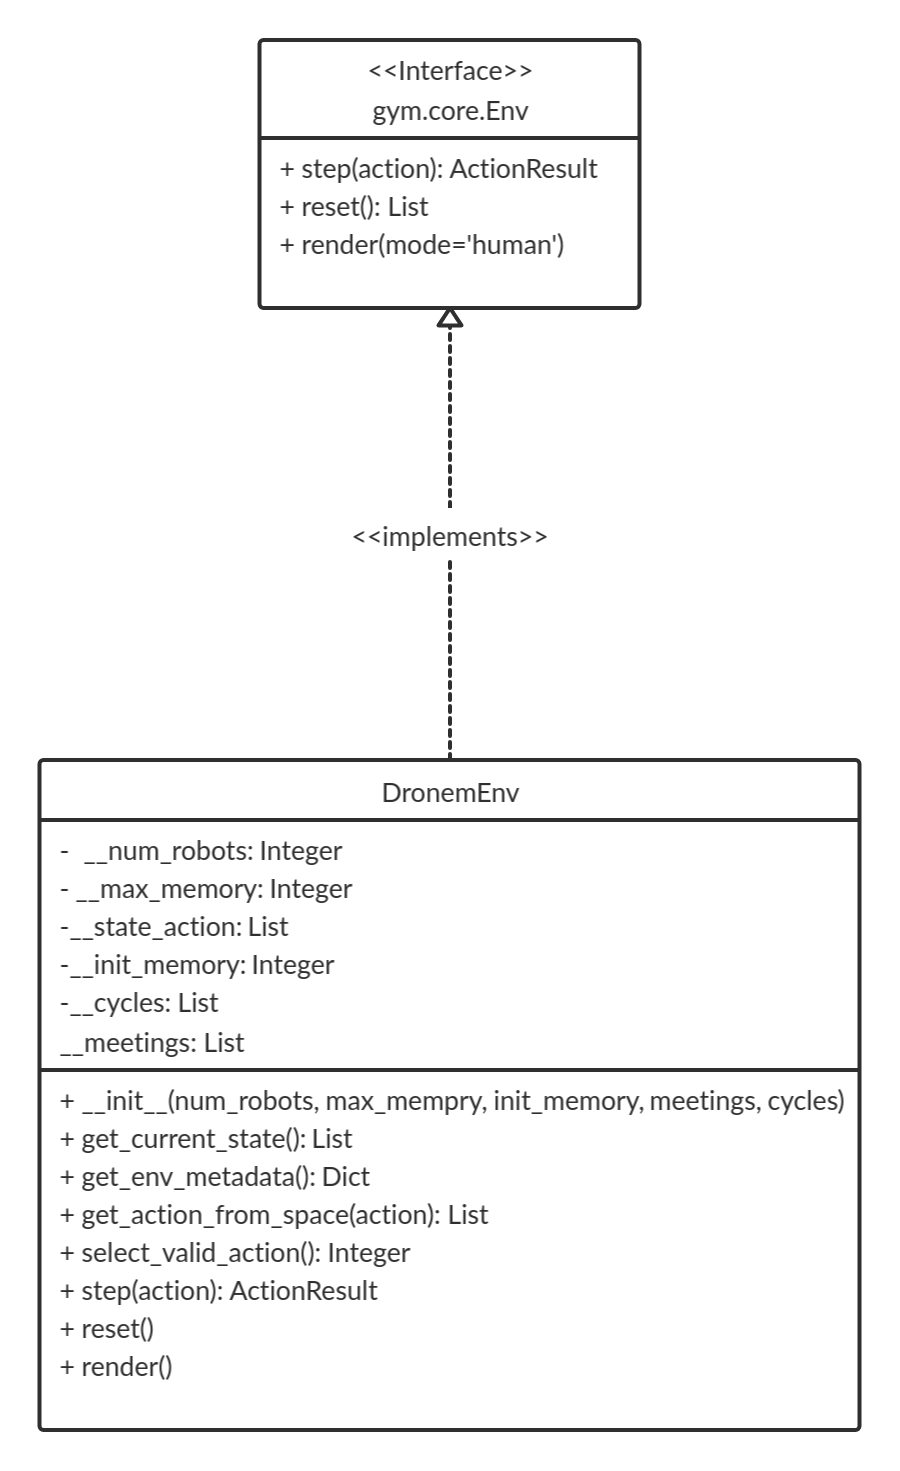
\includegraphics[scale=0.2]{Figures/gymEnvArchitecture.jpg}
    \caption{Dronem environment Gym architecture}
    \label{fig:dronemEnvGym}
\end{figure}{}


\subsection{Advantages and Disadvantages}

In the past, one of the problems in the reinforcement learning community was the lack of benchmarking tools, often the researchers were forced to code their own environments, and because no common interface was used, it was very hard for a research team to apply a reinforcement learning algorithm on environments created by others. 
\par This problem was solved by OpenAI Gym by not only exposing a common interface between all reinforcement learning environments, but also by offering more interesting environments as benchmarks such as the Atari Games. Even more, Gym offers a standardized test bed for algorithms in academic publishing.
\par The only inconvenience exposed by OpenAI Gym is the fact that only episodic reinforcement learning environments can be used, therefore for some environments a series of constraints have to be applied, while in the same time some RL classes of algorithms may not be suitable for episodic environments.

\section{Implementation}\label{implementation}
The implementation phase plays a major role in the life cycle of a software application, because big decisions are made in important aspects such as testing methodologies and development technologies. We will focus more on implementation aspects along this section.

\subsection{Backend}\label{BE}
Backend refers to any part of a software which is not accessible by the user and it is usually composed of a server which, together with an application acts as an operation manager and a database for storing application data. Backend technologies consist of a programming language, in our case \emph{Python}, and usually the programming language which is going to be used for development is enhanced by various frameworks such as \emph{Django}.

\subsection{Django vs Flask}

In recent years many web development frameworks for Python have been released, but none of them are nearly as popular as Django \cite{django} and Flask \cite{flask}. 
Django is an well-established framework having a bigger community of active users as it can be seen in Figure \ref{fig:DjangovsFlask}\cite{flaskvsdjango}, while Flask is a lightweight web framework.

\begin{figure}[!htb]
    \centering
    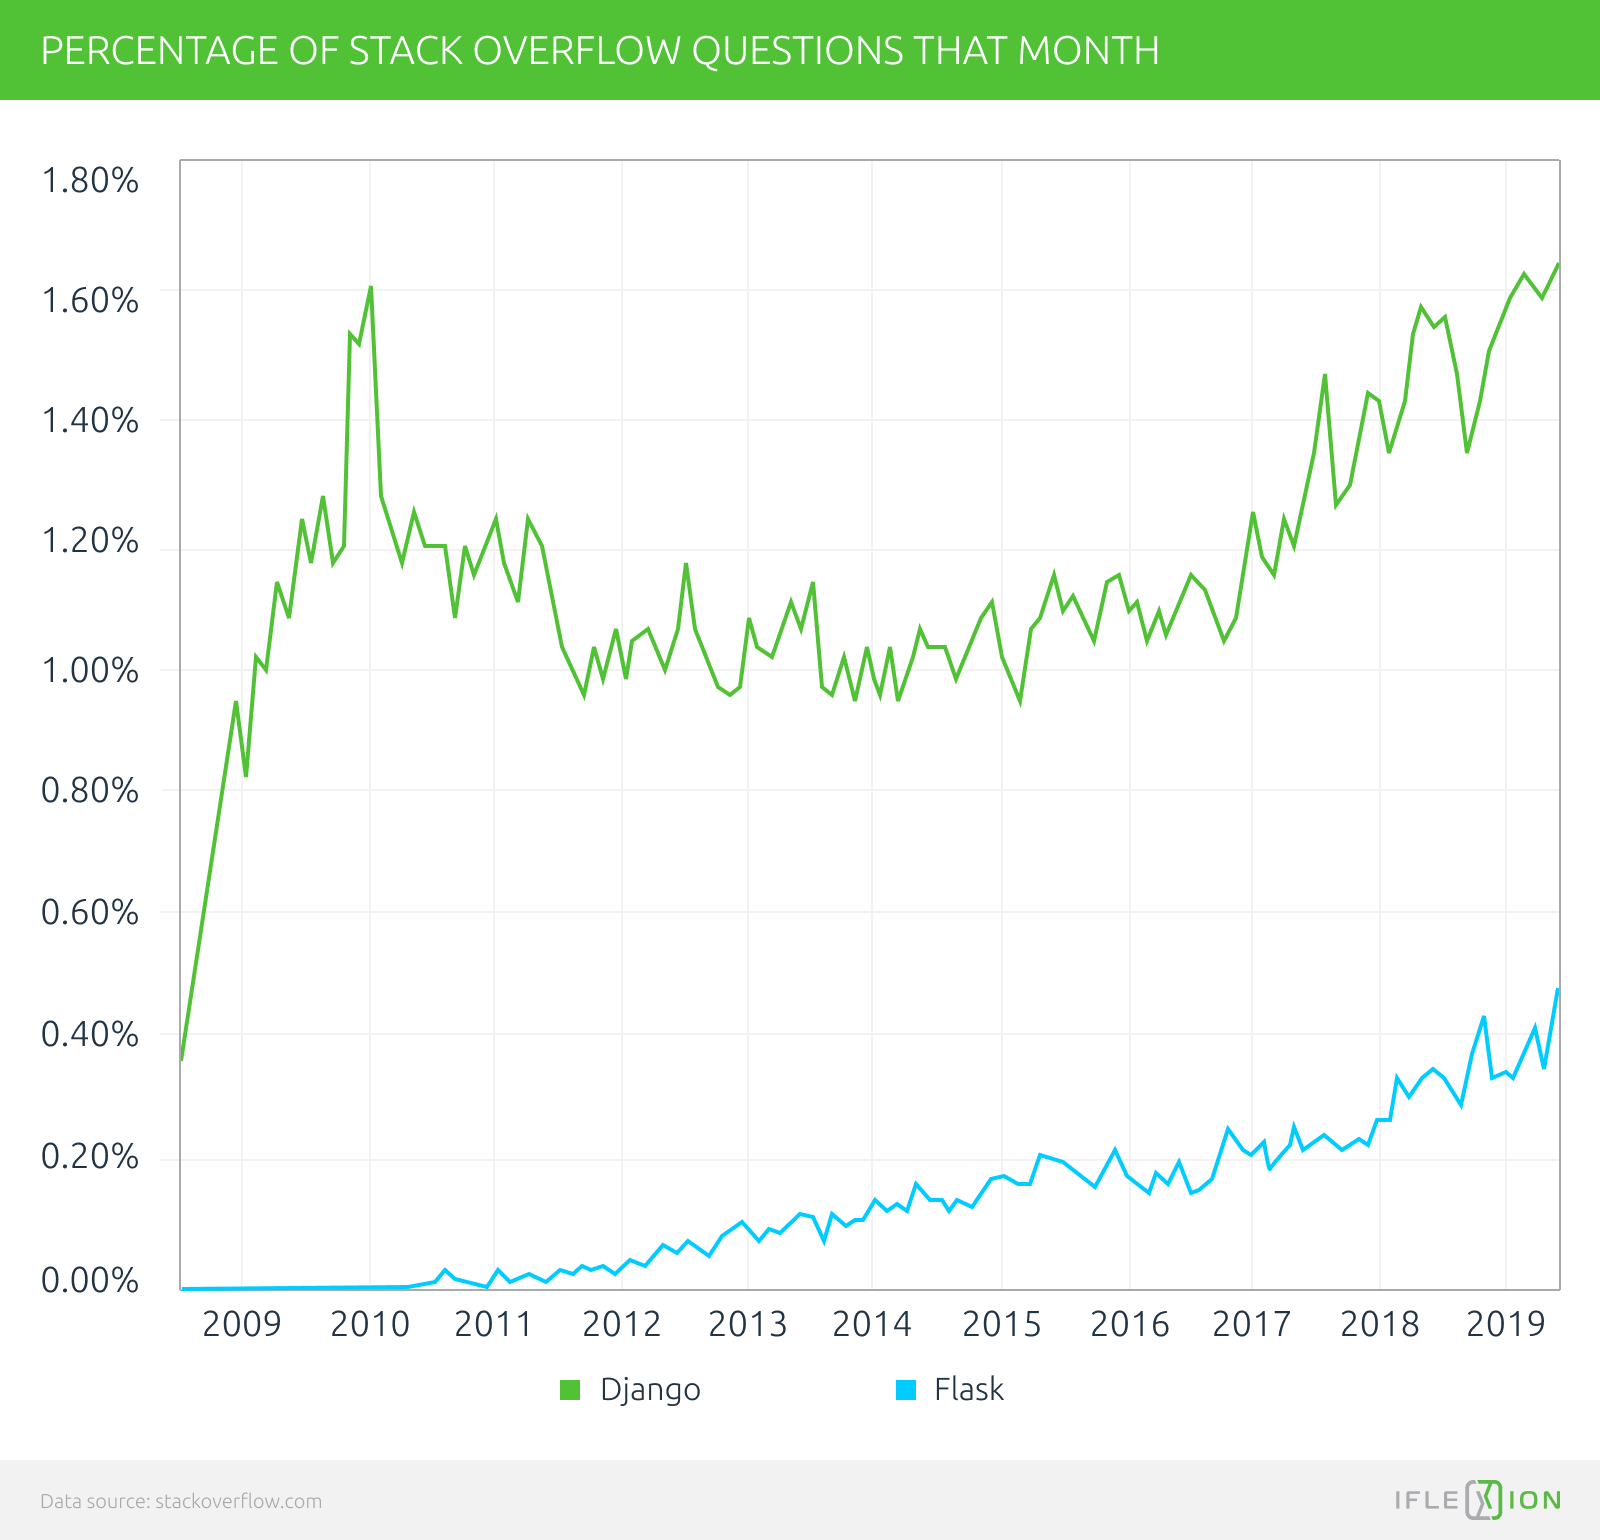
\includegraphics[scale=0.2]{Figures/djangovsFlask.png}
    \caption{Number of StackOverflow questions for Django and Flask}
    \label{fig:DjangovsFlask}
\end{figure}{}


\par Unlike Flask, Django has a 'battery included' philosophy, meaning that all you need in order to fully develop a web application is already included in the framework. Django makes it easier to handle common project administration tasks, by providing a fully functional admin interface, in order for the same functionality to be achieved using Flask, more packages needs to be installed and configured. Another advantage of Dajngo over Flask is allowing the developers to take advantage of a robust object-relational mapping (ORM) mechanism. The developers can use the ORM provided by Django to work with many popular databases such as MySQL, Oracle, SQLite, PostgresSQL whereas in Flask there is no ORM system built in. Flask requires developers to work with databases and perform database operations through SQLAlchemy \cite{sqlalchemy}.
\par Another argument which favors Django over Flask is the fact that developers can divide an application into multiple subapplications, hence it become easier for the developers to integrate new features into the application by splitting work and even reuse subapplications in other projects. Flask requires developers to create each project as a single application, however there is the option do add multiple models and views to the same application. When it comes to testing, both Django and Flask can use the Python integrated unittest framework, and both can be configured to use a secondary solution as necessary. However, the Django's integrated automated testing feature is a strong argument in its favor, especially when there is a need to create tests using dummy databases, as in Flask such a configuration is not trivial to accomplish.
\par As a conclusion, in order to build the Dronem Web application Django is the chosen framework because it offers many ways of creating scalable web applications through its ease of use, robustness, testing versatility and very active community.

\subsection{Django REST Framework}
While Django alone is sufficient in order to develop a scalable web application, in order to enhance it with the latest capabilities of manipulating and serializing data, Django REST Framework (DRF) will be used.
\par Django REST Framework \cite{drf} is a very powerfol toolkit for building Web Application Programming Interfaces (APIs). One of the biggest reasons to use DRF is that it makes it very easy to serialize data. The Django ORM is already a powerful tool for handling database migrations and queries, but it is not that easy to convert entities stored in the database to more used formats such as JavaScript Object Notation (JSON). This is the problem that DRF solves, by easing the conversion of objects stored in the database in formats such as JSON with just a few lines of code.

\subsection{Database}
These days, there is a big debate regarding the database type you should use for your project. Depending on what kind of data your application manages, there are SQL databases and NoSQL databases. For choosing what type of database is suitable for an application, the question "Is the data relational or not?" must be answered. Because our data is highly relational, we chose to use MySQL \cite{MySQL} as database, the following database schema is proposed for the Dronem Web application in Figure \ref{fig:dataBaseSchema}.


\begin{figure}[!htb]
    \centering
    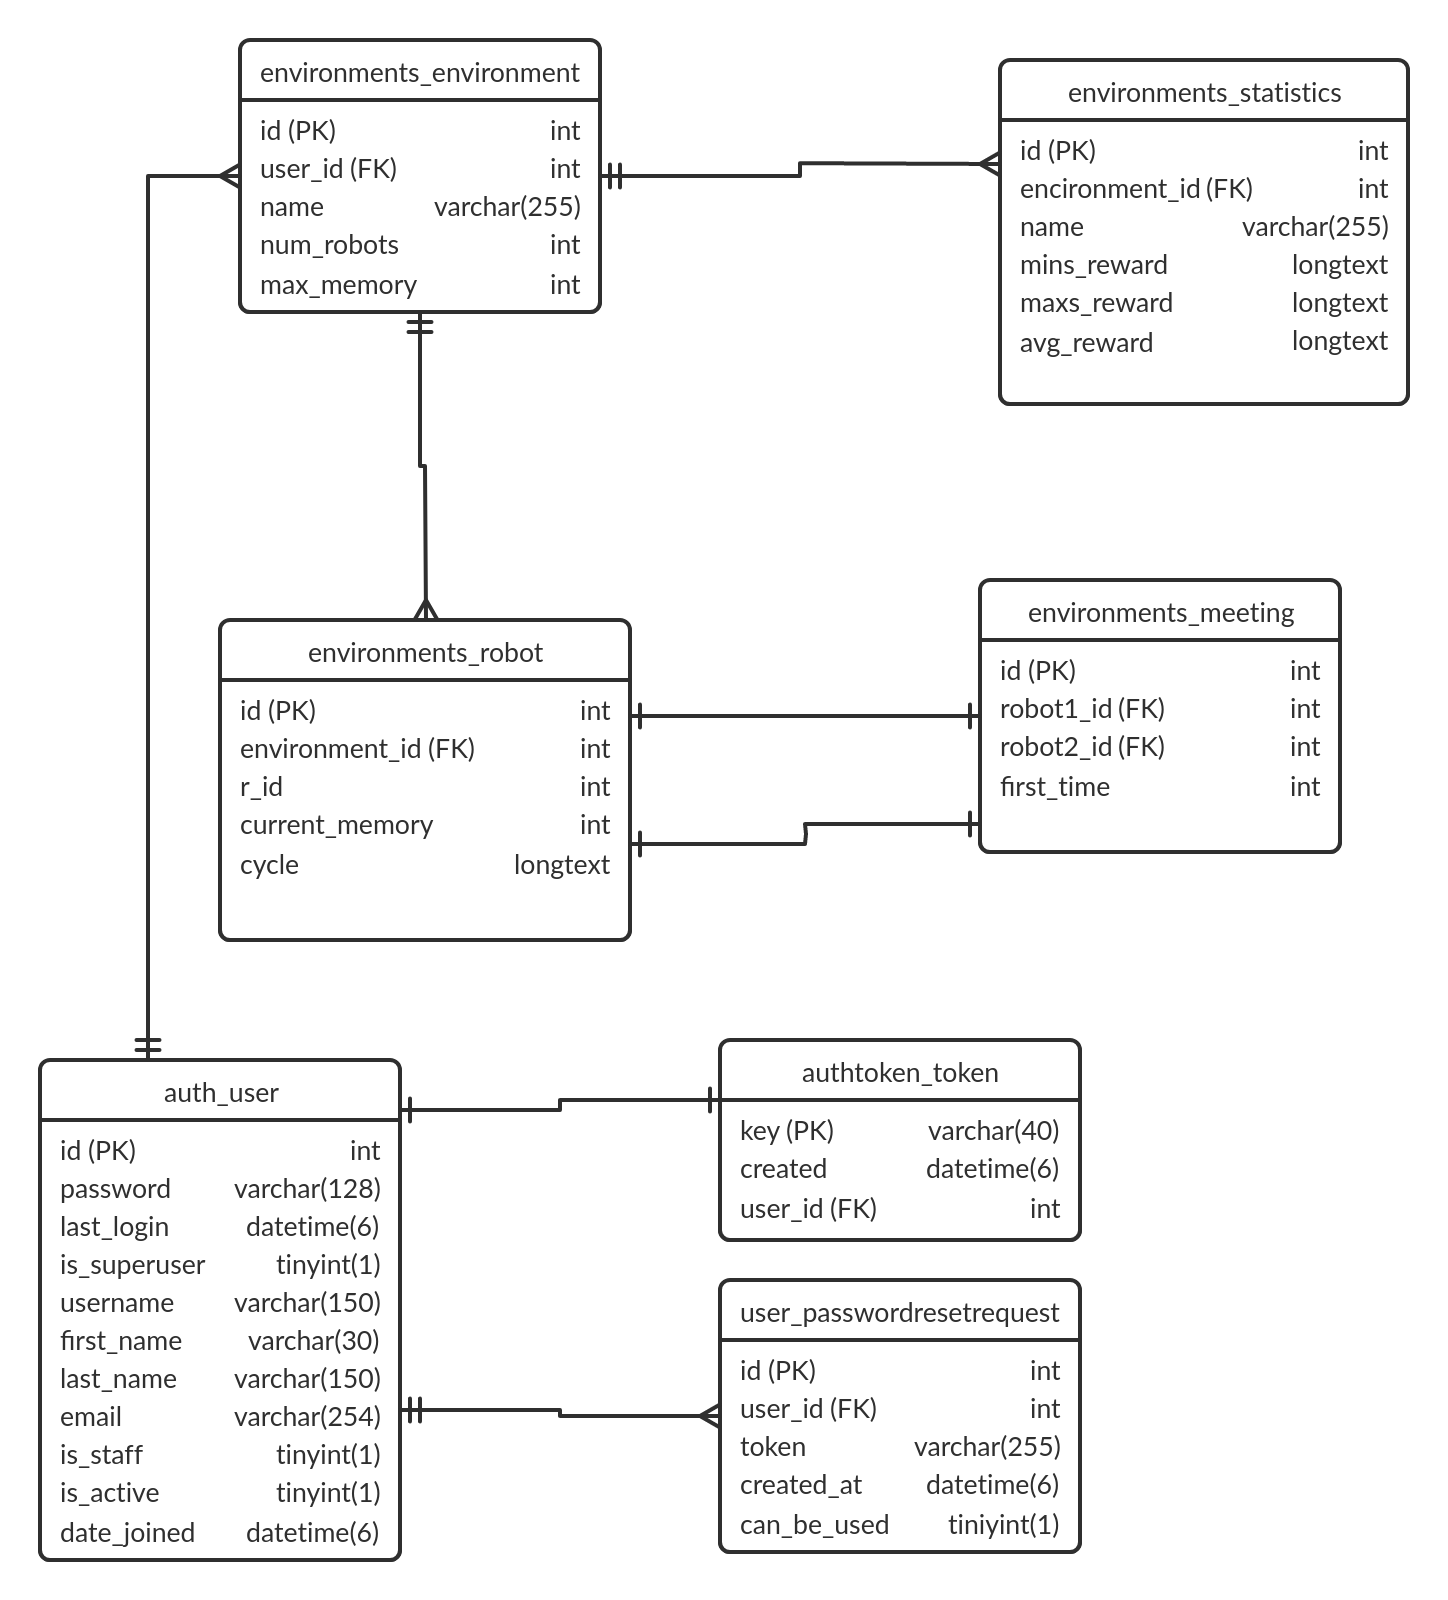
\includegraphics[scale=0.2]{Figures/databaseDiagram.jpg}
    \caption{Dronem Web database schema}
    \label{fig:dataBaseSchema}
\end{figure}{}

\subsection{Frontend}\label{FE}
As opposed to backend, the frontend side of a web application is concerned with the parts of the application which the user can see. The main tools used in frontend development are:
\begin{itemize}
    \item Hyper Text Markup Language (HTML) which is the backbone of any website. Being a markup language it means that it indicates that text can be turned into images, tables or other representations.
    \item Cascading Style Sheets (CSS) which controls the presentation aspect of the site.
    \item JavaScript which is an event-based imperative programming language used to add dynamic interactions to a website, while also maintaining communication with the backend side of the application.
\end{itemize}
\par The JavaScript language which is the most used programming language for frontend side applications, is usually enhanced using various frameworks and libraries such as the one used for the \emph{Dronem Web} frontend ReactJS \cite{react}. We chose ReactJS as our frontend library for JavaScript because it is proven to be highly scalable and extensible by maintaining several big web applications such as Facebook, Dropbox or Tesla.
\subsection{Design choices}

\subsubsection{REST vs GrapQL}
REpresentational State Transfer (REST) \cite{rest} is the most popular web architectural style providing a standard way of communication between computers on the web. Systems which use REST communication are often called RESTful. In order for an interface to be called RESTful the following requirements need to be meet:
\begin{itemize}
    \item Separation between client and server - the interface must separate the concerns of the client (frontend) and server (backend), by doing this the same interface may be used across multiple platforms and the server is more scalable by simplifying its components.
    \item Stateless - requests coming from the client must contain all the information needed in order to fulfill that request, and cannot be directly based on previous requests. 
    \item Cacheable - every response needs to be labeled as being cacheable or not as the client can use that response for future equivalent requests.
    \item Uniform interface - Applying software engineering guidelines, having an uniform interface, the overal complexity of the system is minimized.
    \item Layered system - The architecture of the system must be composed as an hierarchical structure.
\end{itemize}

\par GraphQL\cite{graphQL} on the other hand is a query language for an API and a server-side runtime for executing queries by using a type system defined for the application data. It was created by Facebook and it is supposed to fundamentally change the way applications communicate  across the web. GraphQL promises to solve the main problems which arise from using REST, such as over and under data fetching. Over-fetching means downloading unnecessary data, which is a common problem encountered when using REST, because a REST endpoint can only return fixed data structures. Returning fixed data structures also causes under-fetching, for example think about making a call to retrieve a list of users, then for every user we have to make another request to retrieve their followers. This problems are solved by GraphQL with an ingenious solution, declaring specific queries, which give no more, no less, but the necessary data. 

\par Because GraphQL is still an emerging technology, we chose to use REST for the Dronem Web application, but as more and more documentation and applications using GraphQL will start to appear, we will consider enhancing our application by replacing the RESTful interface with GrapQL.

\subsubsection{Redis}

Redis (REmote DIcrionary Server) \cite{redis} is an open source in-memory data-structure, used as a database, message broker and cache. At a high level Redis can be viewed as key-value database, each value is mapped by a key.
It supports various types of data structures such as strings, hashes, sets, lists, sorted sets etc. Values can only be retrieve it its key is known.
Once installed in a server Redis is very easy to operate using Redis Command Line Interface (CLI), having the following main features:

\begin{itemize}
    \item Speed - Redis is capable of loading a whole dataset in memory, approximately 81.000 GETs/second.
    \item Many Supported Languages - There are many programming languages which support Redis bindings by default.
    \item Master/Slave Replication - Redis supports a very simple and fast Master/Slave replication, being so simple that in only needs one line of configuration.
\end{itemize}

The main reason Redis has been chosen to be the message broker for the Dronem Web application is that it has a different evolution path in the key-value databases where values can store more complex data types such as our training configurations for environments, with atomic operations on those complex data types.

\subsubsection{Celery}
Celery \cite{celery} is a task queue (mechanism to distribute work across machines) used in Django. Its main use cases are:
\begin{itemize}
    \item Tasks that need to run asynchronously.
    \item Heavy background computations.
    \item Periodic tasks.
    \item Interaction with external API's.
\end{itemize}

\par Celery communicates via messages, using a broker such as Redis or RabbitMQ, whose goal is to mediate between clients and workers. In order for the client to initiate a task, the client adds a messages into the queue, then the broker assigns the message to a worker. After the worker finishes its job the effects of the task are stored in a task store result, in our case the database.

\par Because training an environment is not an instantaneous task we want to exclude the process from the request-response HTTP cycle. In order to achieve this, whenever a user requests an environment training a Celery task is started so that a user can train multiple environments in the same time while also being able to use other features of the application because it is not limited by the request-response HTTP cycle (i.e. the user does not need to wait until the training process is complete in order to use the application).

\subsection{Testing}
Following the software development methodology stated in Section \ref{softDev}, one of the most important activities is testing, as most of the time software testing determines the quality of software after a programmer develops it. The testing process involves evaluating information that is related to a product. Also testing ensures that the application satisfies the security requirements in order to protect confidential data.
\par While there are many software testing techniques and procedures we choose to use testing based on specification (Black Box Testing) and testing based on implementation (White Box Testing). Combining the two mentioned techniques in practice yields the best results, by using the Equivalence Class Partitioning (ECP) and Boundary Value Analysis (BVA) from Black Box Testing and Cyclomatic Complexity (CC) and the coverage criteria from White Box Testing.
\par In order to create flexible and easy to write tests the Pytest\cite{pytest} framework was used. Pytest is a framework which allows to write Python tests for different application levels including database, API or User Interface (UI). One of the most important advantages of Pytest over other testing frameworks is the ease of use and test readability, which are key features when it comes to testing.
What differentiate Pytest from other testing frameworks is the usage of a system based on fixtures (functions which initialize test functions), instead of using the classic \emph{setUp}, \emph{tearDown} testing system.
Another important feature of Pytest is the ease of creating \emph{mock} objects using a special fixture, called \emph{monkeypatch}, which allows changing the behaviour of any Python object with only one line of code.

\par For the Dronem Web application, several tests were designed and implemented in order to ensure that the application works according to the system requirements defined in Section \ref{ad}. Extensive testing was done around the \emph{QLearning} algorithm and the \emph{DronemGymEnv} architecture, while numerous tests were conducted for the API of the application in order to ensure optimal functionality.
\subsection{Documentation}
Documenting application is a mandatory activity in software development because good documentation makes it easier for the developers to maintain and add new features to the application. The main focuses of a documentation are development, maintenance and knowledge transfer to other developers. Usually the principal components of a documentation concern with server environments, databases, troubleshooting, application installation and code deployment.
\par The documentation for the \emph{Dronem Web} application is composed of two main parts. The first part consists in detailed comments for every relevant function, including input parameters, requirements and effects. Also detailed comment blocks were written for the \emph{DronemGymEnv} environment highlighting the main characteristics of the environment. The second part of the documentation is represented by the API documentation which was automatically generated using Django REST Swagger. An example of the API documentation generated for one REST \emph{/users/signin/} path can be saw in Figure \ref{fig:apiDoc} 

\begin{figure}[!htb]
    \centering
    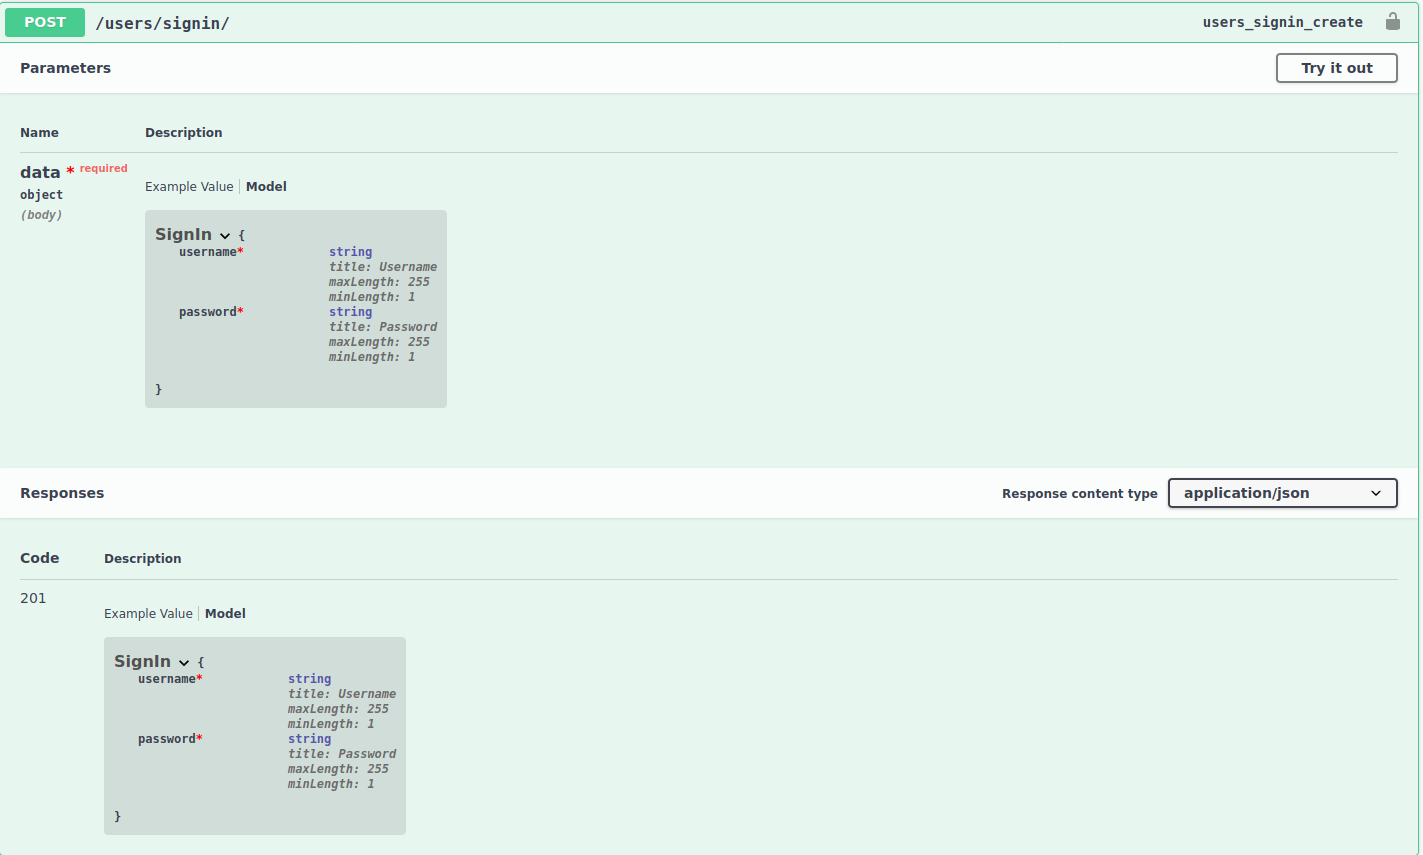
\includegraphics[scale=0.3]{Figures/apiDoc.png}
    \caption{API documentation for \emph{/users/signin/} path}
    \label{fig:apiDoc}
\end{figure}{}

\section{User manual}\label{userManual}
It is very important to write a good User Manual of the application in order to ease the first interactions of the user with the main functionalities of the platform, hence this section is focused on familiarizing the user with the application.

\subsection{Creating environments}
To achieve creation of an environment the user must click the Add Environment tab in order to to have access to the environment add form shown in Figure \ref{fig:addEnv}.
After that, the user can choose between adding the environment through a JSON file or by completing the multi-step form, of course the preferred way is via a JSON file, as adding a big environment by hand using a form is a tedious work. After completing the multi step form, or uploading the JSON file, an \emph{Add Environment} button will appear, clicking it will result in creating a new environment.


\begin{figure}[!htb]
    \centering
    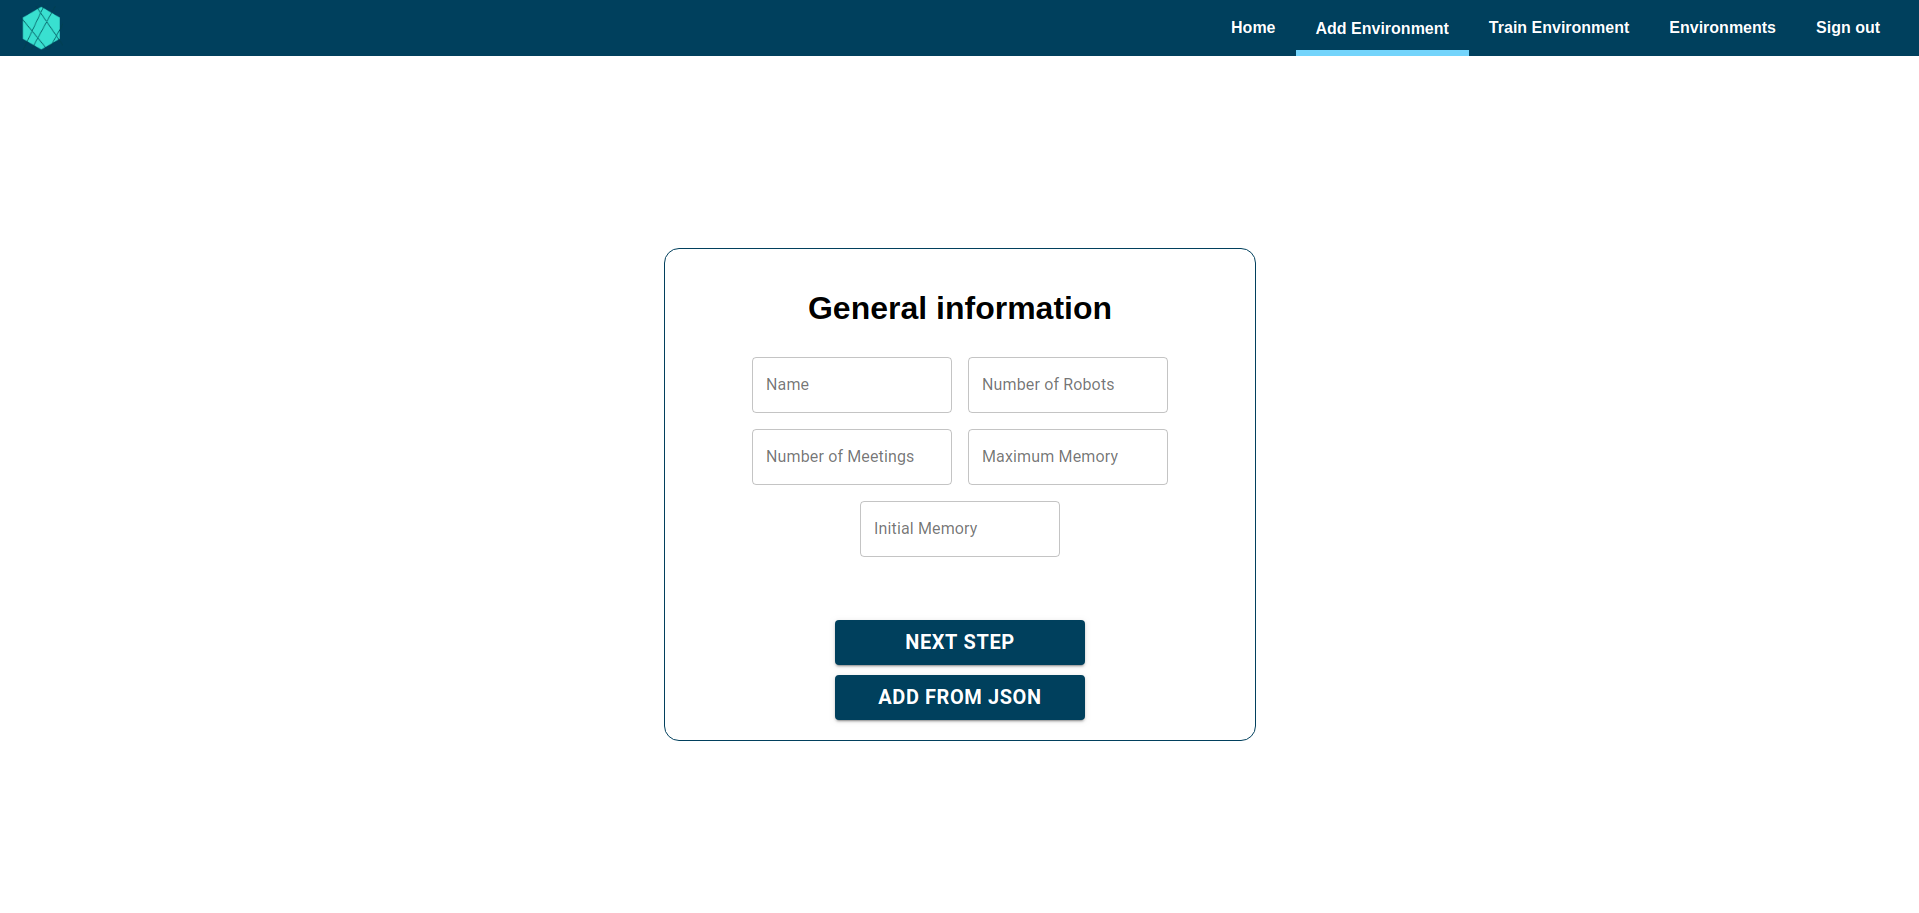
\includegraphics[scale=0.22]{Figures/addEnvsView.png}
    \caption{Drone Web add environment view}
    \label{fig:addEnv}
\end{figure}

\subsection{Training environments and downloading Q-tables}
\subsubsection{Training an environment}
In order to start a training session, the user must select the \emph{Training Environment} tab. After clicking the training tab, the screen shown in Figure \ref{fig:trainView} will appear, the user must select an environment and input the training parameters for the algorithm. Finally clicking the Train button will start a training session, and live statistics of the training will appear on the canvas situated on the right side of the screen.

\begin{figure}[!htb]
    \centering
    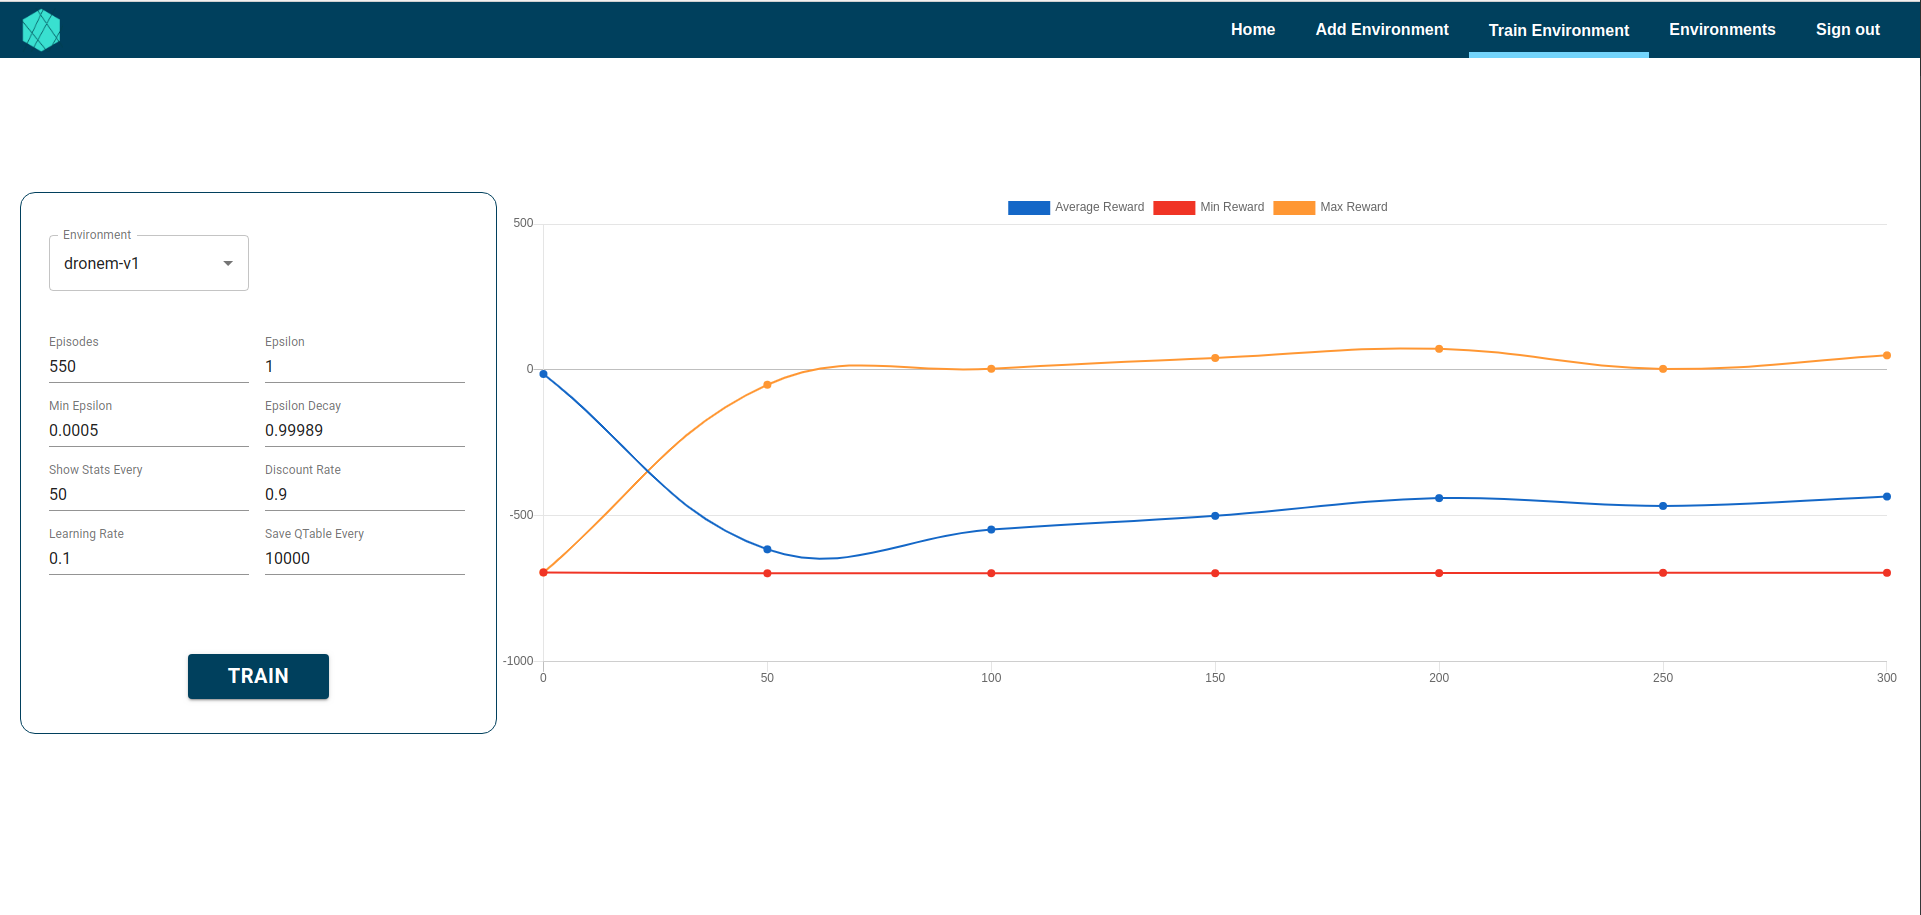
\includegraphics[scale=0.22]{Figures/trainView.png}
    \caption{Drone Web train view}
    \label{fig:trainView}
\end{figure}


\subsubsection{Downloading Q-tables}
The environments tab, presents numerous functionalities as can be observed in Figure \ref{fig:ensvView}. The user can download a JSON file containing the best Q-table for an environment by clicking the \emph{Download Best QTable} button. 

\begin{figure}[!htb]
    \centering
    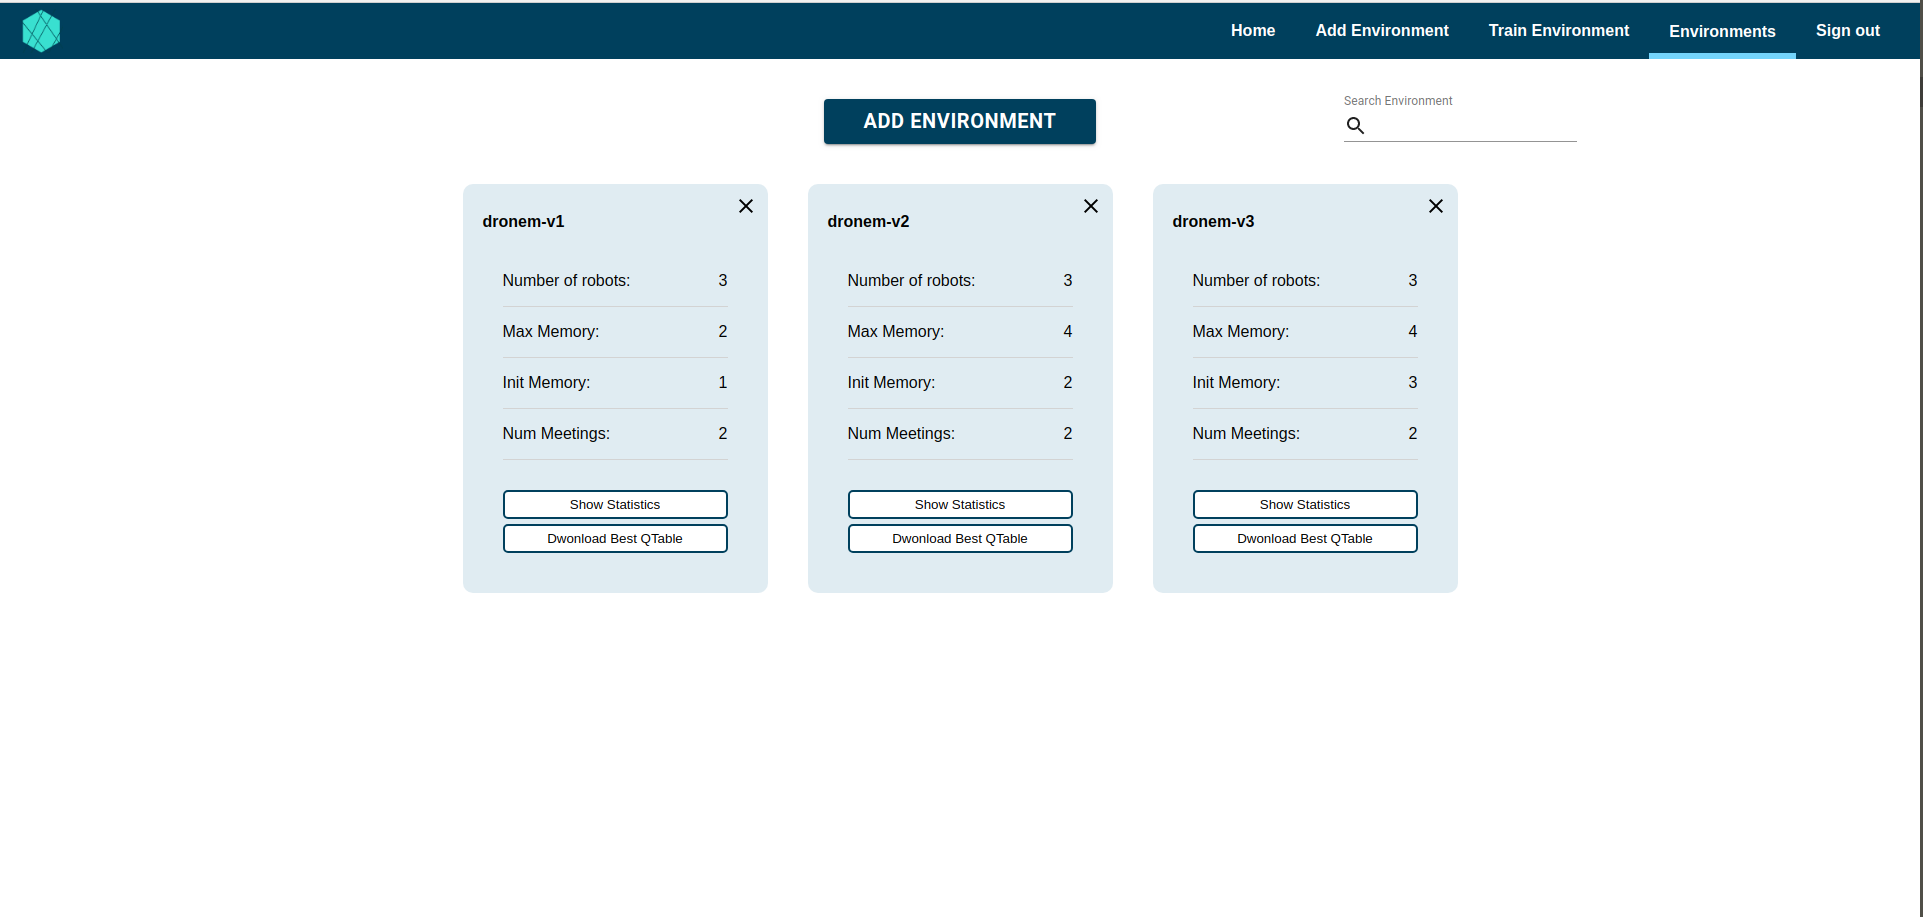
\includegraphics[scale=0.22]{Figures/environmentsView.png}
    \caption{Drone Web environments view}
    \label{fig:ensvView}
\end{figure}

\subsubsection{Showing training statistics}
Also the user can retrieve statistics about past training of an environment, by clicking the \emph{Show Statistics} button, leading to the view depicted in Figure \ref{fig:statisticsView}


\begin{figure}[!htb]
    \centering
    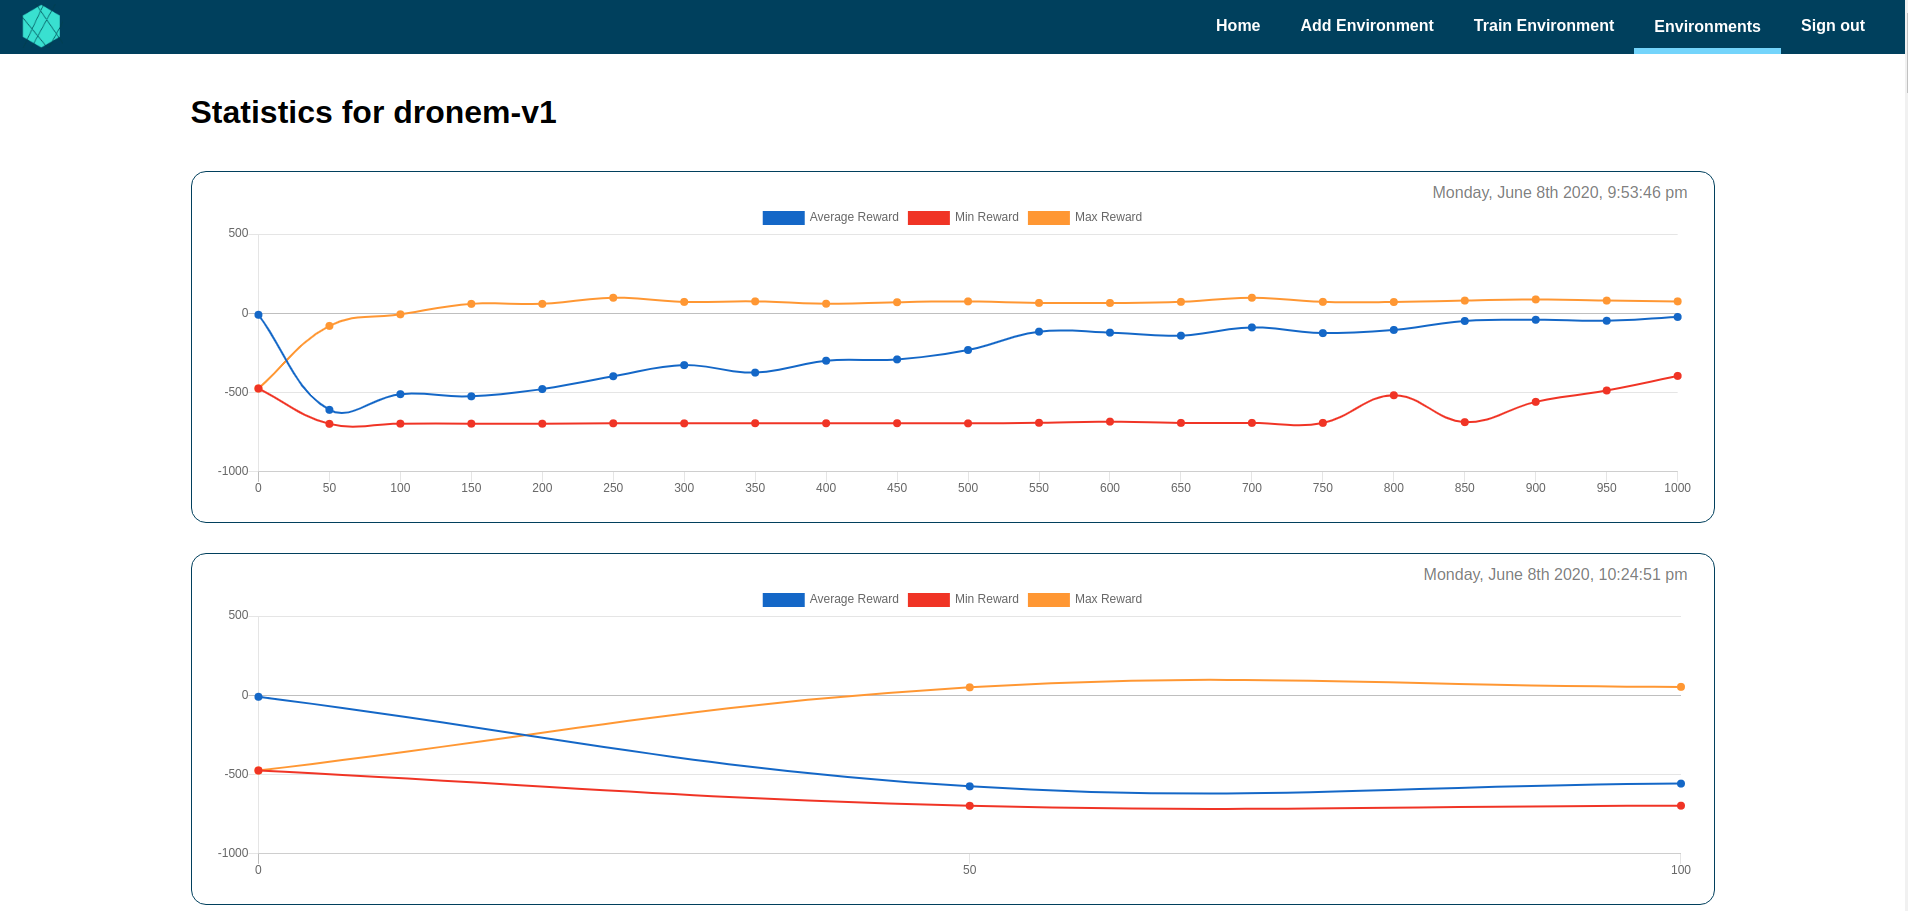
\includegraphics[scale=0.22]{Figures/statisticsView.png}
    \caption{Drone Web statistics view}
    \label{fig:statisticsView}
\end{figure}


\section{Discussion}\label{softDiscussionn}
The purpose of this chapter was to present the software development process followed in order to develop the \emph{Dronem Web} application. Several development activities were documented along this chapter, starting with analysis and design, implementation, testing and documentation of the application while outlining the importance of following a software development methodology when constructing an application and what catastrophic consequences can arise when no strategy is used. This section presents the original contributions and benefits brought to the Reinforcement Learning community by the creation of this application.

\par First of all the \emph{Dronem Web} is, to the best of our knowledge, the only application available for creating, manipulating and training MRP environments. We presumably think that more and more users will start using our application for different tasks ranging from university level projects to real world problems such as smart surveillance systems, as long as there is a suitable MRP modelling for those problems. Another original contribution of our application consists in the possibility to retrieve the Q-table for the best training session of an environment, hence the training results can be further used in real applications that are modelled as MRP problems. Also we encourage the users to further extend our \emph{Dronem Gym Environment} which will be publicly available at: \url{https://github.com/GeorgianBadita/Dronem-gym-envirnoment}. We hope to grow a flourishing community of RL enthusiasts around our application who will further develop the foundation presented by this thesis.

\par Being constructed with the latest technologies and with the best software development practices, we believe the Dronem Web application to be very scalable, being able to handle many users and training sessions in parallel if deployed on capable enough hardware.

\section{Future enhancements}\label{futureEnh}
 This application is laid as a foundation for an efficient way to create, manipulate and train MRP environments, but it opens up several paths for future enhancements.

\par As every application strives to be better and better, we think that our application may benefit from  some enhancements too. First of all, the application is limited in the types of environments it can manage, users are able to only create and train environments corresponding to the specification defined in Chapter \ref{flow}. In the future we are going to add the possibility to manipulate different types of environments or even create environments for different reinforcement learning problems.

\par When it comes to training times, currently for some environments waiting times are very high, due to the fact that the application runs on a computer with low system specifications. A possible solution to overcome this issue would be to deploy the backend of the application on a much more powerful machine, reducing training times significantly, for example an EC2 Amazon Web Services (AWS) instance can be used. A task framework solution has already been implemented in order to reduce training times, but as python is not a 'real' multithreaded programming language, because of its Global Interpreter Lock (GIL), other solutions need to be taken into consideration.

\par Another important area where the Dronem Web application can be improved is the crash recovery. If the machine where the backend of the application is stored crashes, or even if the Redis or Celery services stop working all environments which are trained in that moment will stop and every interaction with the application will fail. Hence, a mechanism for crash recovery is also needed to be considered for the application, so that after any service crash all training environments should return to their state before the crash. One solution for this problem would be to save the entire application state in the database whenever a training step is taken, although this would increase training times, it will ensure that the application can recover whenever a something bad happens. Nevertheless more research in this direction is needed and more enhancements will be taken into consideration in the future.